\chapter{Mængdelære}
\label{chap:ch3}

I softwareudvikling arbejder vi hele tiden med samlinger af ting: brugere i et system, poster i en database eller knuder i et netværk. Mængdelæren giver os det formelle matematiske sprog til at beskrive og håndtere disse samlinger præcist og klart. Den er fundamentet for mange centrale begreber i datalogi -- fra databaseforespørgselssprog som SQL til datastrukturer og algoritmisk logik.

Dette kapitel introducerer mængdelærens grundlæggende principper. Vi begynder med den enkle, intuitive idé om en mængde og ser på den formelle notation, der bruges til at definere mængder. Derefter gennemgår vi de væsentligste relationer mellem mængder, fx delmængder, og de centrale operationer, der bruges til at kombinere dem, herunder foreningsmængder, fællesmængder og komplementer. Disse operationer svarer direkte til de logiske operatorer (\texttt{OR}, \texttt{AND}, \texttt{NOT}), der styrer forløbet i din kode. Til sidst ser vi på ordnede samlinger, der kaldes tupler, og introducerer en enkel metode til at bevise, at to mængder er lig med hinanden.

\section{Hvad er en mængde?}
En mængde er en uordnet samling af forskellige objekter. Objekterne i en mængde kaldes dens \textbf{elementer} eller \textbf{medlemmer}. Vi kan tænke på en mængde som en simpel beholder, hvor ting er samlet, og hvor rækkefølgen, vi skriver dem i, ikke har betydning. For eksempel kan mængden af primærfarver skrives som $\{ \text{rød}, \text{gul}, \text{blå} \}$ eller lige så godt som $\{ \text{blå}, \text{rød}, \text{gul} \}$.

Mængder er en hjørnesten i moderne matematik og et grundlæggende begreb i datalogi. De udgør det logiske grundlag for alt fra databaseforespørgselssprog og datastrukturer til specifikationen af typer i programmeringssprog.

% --- Figure Placeholder ---
% This figure illustrates the basic concept of a set.
% It is inspired by Slide 3 of your PowerPoint presentation.
\begin{figure}[htbp]
    \centering
    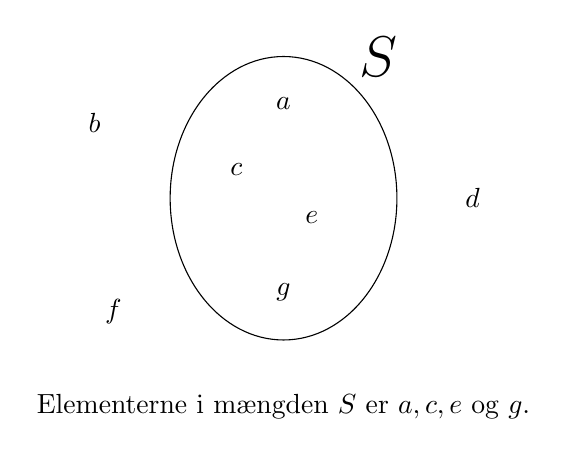
\begin{tikzpicture}[scale=1.2]
        % The set S as an ellipse
        \draw (0,0) ellipse (1.2cm and 1.5cm);
        \node at (1, 1.5) {\huge $S$};
        
        % Elements inside the set S
        \node at (0, 1) {$a$};
        \node at (-0.5, 0.3) {$c$};
        \node at (0.3, -0.2) {$e$};
        \node at (0, -1) {$g$};
        
        % Elements outside the set S
        \node at (-2, 0.8) {$b$};
        \node at (-1.8, -1.2) {$f$};
        \node at (2, 0) {$d$};

        % Annotation
        \node[align=center] at (0,-2.2) {Elementerne i mængden $S$ er $a, c, e$ og $g$.};
    \end{tikzpicture}
    \caption{En mængde $S$ med fire elementer. Objekterne $b, d$ og $f$ er ikke elementer i $S$.}
    \label{fig:set_concept}
\end{figure}

\subsection*{Angivelse af en mængde}
Der er to primære måder at beskrive en mængde på: ved eksplicit at opremse dens elementer eller ved at angive en egenskab, som elementerne skal opfylde.

\subsubsection*{Listenotation}
Den mest direkte måde at definere en mængde på er at opremse alle dens elementer mellem krøllede parenteser, $\{ \}$. Det kaldes \textbf{listenotation}.

For eksempel:
\begin{itemize}
    \item Mængden af alfabetets første fem bogstaver er $A = \{a, b, c, d, e\}$.
    \item Mængden af de første tre positive hele tal er $C = \{1, 2, 3\}$.
    \item En mængde kan indeholde forskellige typer af elementer: $D = \{ \text{Alice}, 42, \pi \}$.
\end{itemize}

Når vi bruger listenotation, gælder der to grundlæggende regler:
\begin{enumerate}
    \item \textbf{Rækkefølgen har ingen betydning.} En mængde er alene bestemt af de elementer, den indeholder, ikke af den rækkefølge, de er opremset i. For eksempel er $\{1, 2, 3\}$ præcis den samme mængde som $\{3, 1, 2\}$.
    \item \textbf{Hvert element skal være entydigt.} Et element er enten med i en mængde, eller også er det ikke. At opremse et element mere end én gang er overflødigt og ændrer ikke mængden. For eksempel er mængden $\{a, a, b, c, c\}$ blot $\{a, b, c\}$.
\end{enumerate}


\subsubsection*{Mængdebyggernotation}
Når det er upraktisk eller umuligt at opremse alle elementer (fx for uendelige mængder), bruger vi \textbf{mængdebyggernotation}. Denne metode definerer en mængde ved at angive en egenskab eller regel, som elementerne skal opfylde. Notationen bruger en lodret streg `|` eller et kolon `:`, som læses »sådan at«.

Den generelle struktur er:
\[ \{ \text{variabel} \mid \text{en egenskab, som variablen skal opfylde} \} \]

For eksempel:
\begin{itemize}
    \item $A = \{ l \mid l \text{ er en vokal i det engelske alfabet} \}$ \\
    Det læses: »$A$ er mængden af alle elementer $l$, sådan at $l$ er en vokal i det engelske alfabet.« Det er en anden måde at skrive $A = \{a, e, i, o, u\}$ på.
    
    \item $C = \{ n \mid n \in \mathbb{Z} \text{ og } 0 < n < 4 \}$ \\
    Det læses: »$C$ er mængden af alle tal $n$, sådan at $n$ er et helt tal, og $n$ er større end 0 og mindre end 4.« Det definerer mængden $\{1, 2, 3\}$.
    
    \item $E = \{ x \mid x \text{ er et lige helt tal} \}$ \\
    Det definerer den uendelige mængde af alle lige hele tal: $\{\dots, -4, -2, 0, 2, 4, \dots\}$.
\end{itemize}

Mængdebyggernotation er meget effektiv, fordi den gør det muligt at definere store, komplekse eller endda uendelige mængder med en kort og præcis beskrivelse.

\section{Vigtige mængder: talsystemerne}
Tal er fundamentet for matematik og beregning. De forskellige kategorier af tal, vi bruger i hverdagen -- fra at tælle ting til at måle kontinuerte størrelser -- kan defineres formelt som mængder. Det er afgørende for enhver softwareingeniør at forstå disse grundlæggende mængder, fordi de ligger til grund for datatyper, aritmetisk logik og numeriske algoritmer.

\subsection*{De vigtigste talmængder}
Følgende mængder er blandt de vigtigste i matematikken og bruges overalt i naturvidenskab og ingeniørarbejde.

\begin{description}
    \item[Naturlige tal ($\mathbb{N}$)] Mængden af positive hele tal, som bruges til at tælle: $\{1, 2, 3, \dots\}$. Nogle gange defineres denne mængde, så den også indeholder $0$. På grund af denne tvetydighed er det ofte tydeligere at angive \textit{positive hele tal} eller \textit{ikke-negative hele tal}.

    \item[Hele tal ($\mathbb{Z}$)] Mængden af alle positive og negative hele tal, inklusive nul: $\{\dots, -2, -1, 0, 1, 2, \dots\}$.

    \item[Rationale tal ($\mathbb{Q}$)] Mængden af alle tal, der kan skrives som en brøk $\frac{p}{q}$, hvor $p$ og $q$ er hele tal og $q \neq 0$. Den omfatter alle hele tal samt alle endelige og periodiske decimalbrøker. Eksempler: $\frac{1}{2}$, $-5$, $0.25$.

    \item[Reelle tal ($\mathbb{R}$)] Mængden af alle tal på tallinjen. Den omfatter både rationale tal og irrationale tal (som $\pi$ eller $\sqrt{2}$), der ikke kan skrives som simple brøker.
    
    \item[Komplekse tal ($\mathbb{C}$)] Mængden af alle tal, der kan skrives på formen $a + bi$, hvor $a$ og $b$ er reelle tal, og $i$ er den imaginære enhed, som opfylder $i^2 = -1$.
\end{description}

Det er vigtigt at kunne visualisere relationerne mellem disse mængder for at forstå dem. Et Venn-diagram viser hierarkiet i, hvordan mængderne ligger inden i hinanden, mens en tallinje illustrerer, hvordan de dækker eller udfylder kontinuummet af værdier.

% --- Venn Diagram of Number Systems ---
% This is the TikZ code you provided for the number system Venn diagram.
\begin{figure}[htbp]
    \centering
    % Shared diagram of the principal number sets.
% The part of R outside Q is exactly R \setminus Q; it is not a separate oval.
\begin{tikzpicture}[scale=0.7]
    % Complex numbers (outer set)
    \draw[thick, fill=mseComplex!35] (-12,-6) rectangle (10,5);
    \node at (8,4) {\Huge $\mathbb{C}$};

    % Real numbers. The area not covered by Q is the irrational numbers.
    \draw[thick, fill=mseReals] (-4,0) ellipse (7.8cm and 4.5cm);
    \node at (-3,3.8) {\Large $\mathbb{R}$};

    % Rational numbers and their nested subsets
    \draw[thick, fill=mseRationals] (-7,0) ellipse (4.5cm and 3cm);
    \node at (-11,0) {\Large $\mathbb{Q}$};

    \draw[thick, fill=mseIntegers] (-7,0) ellipse (3cm and 2cm);
    \node at (-9.5,0) {\Large $\mathbb{Z}$};

    \draw[thick, fill=mseNaturals] (-7,0) ellipse (2cm and 1.2cm);
    \node at (-7,0) {\Large $\mathbb{N}$};

    % These labels identify the two complementary regions.
    \node[align=center] at (0.7,0)
        {\Large $\mathbb{R}\setminus\mathbb{Q}$\\[-1pt]
         \small Irrationale tal};
    \node[align=center] at (7,0)
        {\Large $\mathbb{C}\setminus\mathbb{R}$\\[-1pt]
         \small Ikke-reelle komplekse tal};
\end{tikzpicture}

    \caption{Et Venn-diagram, der illustrerer den hierarkiske relation mellem de vigtigste talmængder.}
    \label{fig:venn_num}
\end{figure}

\begin{remark}
    Venn-diagrammet i \autoref{fig:venn_num} viser, at mængden af reelle tal ($\mathbb{R}$) udelukkende består af rationale ($\mathbb{Q}$) og irrationale tal. Der findes intet reelt tal, som hverken er det ene eller det andet. Derfor betegnes mængden af irrationale tal formelt $\mathbb{R} \setminus \mathbb{Q}$, hvilket betyder »mængden af alle reelle tal bortset fra de rationale tal«.
\end{remark}

% --- The Number Line ---
% This figure is inspired by Slide 9 of your PowerPoint presentation.
\begin{figure}[htbp]
    \centering
    \begin{tikzpicture}[
        every node/.style={font=\small},
        axis/.style={->, thick},
        tick/.style={black, thick},
        dot/.style={circle, fill, inner sep=1.5pt},
        integer/.style={circle, fill=mseDarkText, inner sep=1.5pt},
        rational/.style={circle, fill=mseOrange, inner sep=1.5pt},
        irrational/.style={circle, fill=mseQuestionBorder, inner sep=1.5pt}
    ]
        % Axis line
        \draw[axis] (-4.5,0) -- (4.5,0) node[right]{$\mathbb{R}$};
        
        % Ticks and labels for integers
        \foreach \x in {-4,...,4}{
            \draw (\x, 0.1) -- (\x, -0.1);
            \node[below] at (\x, -0.3) {\x};
            \node[integer] at (\x, 0) {};
        }

        % Annotations for different number sets (properly spaced)
        \node[above=20pt, color=orange!70] at (0,0) {Hele tal ($\mathbb{Z}$) er markeret med prikker.};
        
        % Example rational numbers
        \node[rational] at (2.5, 0){};
        \node[above=3pt] at (2.5, 0){$\frac{5}{2}$};
        \node[rational] at (-1.5, 0){};
        \node[above=3pt] at (-1.5, 0){$-\frac{3}{2}$};
        \node[below=15pt, color=mseOrange] at (0.5,-0.3) {Rationale tal ($\mathbb{Q}$) udfylder brøkerne.};
        
        % Example irrational numbers
        \node[irrational] at (1.414, 0){};
        \node[above=3pt] at (1.414, 0){$\sqrt{2}$};
        \node[irrational] at (-3.141, 0){};
        \node[above=3pt] at (-3.141, 0){$-\pi$};
        \node[below=30pt] at (0,-0.3) {\textcolor{mseQuestionBorder}{Irrationale tal udfylder hullerne} \textcolor{mseViaBlue}{og fuldender den reelle tallinje.}};
        
    \end{tikzpicture}
    \caption{Den reelle tallinje, udfyldt med hele tal, rationale tal og irrationale tal.}
    \label{fig:number_line}
\end{figure}


\subsection*{Intervalnotation}
I mange anvendelser har vi brug for at henvise til et sammenhængende udsnit af de reelle tal. \textbf{Intervalnotation} er en praktisk kortform til at beskrive sådanne delmængder af $\mathbb{R}$.

Et interval er bestemt ved sine to endepunkter. Vi bruger firkantede parenteser `[` `]` til at angive, at et endepunkt er med i mængden, og runde parenteser `(` `)` til at angive, at det ikke er med.

\begin{description}
    \item[Lukket interval:] Indeholder begge endepunkter.
    \[ [a, b] = \{ x \in \mathbb{R} \mid a \leq x \leq b \} \]

    \item[Åbent interval:] Indeholder ingen af endepunkterne.
    \[ (a, b) = \{ x \in \mathbb{R} \mid a < x < b \} \]

    \item[Halvåbne intervaller:] Indeholder det ene endepunkt, men ikke det andet.
    \[ [a, b) = \{ x \in \mathbb{R} \mid a \leq x < b \} \quad \text{og} \quad (a, b] = \{ x \in \mathbb{R} \mid a < x \leq b \} \]
\end{description}

\begin{example} Intervalnotation
\begin{itemize}
    \item $[-2, 3]$ er mængden af alle reelle tal fra $-2$ til $3$, inklusive $-2$ og $3$.
    \item $(-2, 3)$ er mængden af alle reelle tal mellem $-2$ og $3$.
    \item $[0, 100)$ betegner alle tal fra $0$ op til (men ikke med) $100$.
\end{itemize}
\end{example}

Intervaller kan også være ubegrænsede, så de strækker sig mod plus eller minus uendelig ($\infty$). Da uendelig ikke er et tal, udelukkes det altid med en rund parentes.
\[ (a, \infty) = \{ x \in \mathbb{R} \mid x > a \} \quad \text{og} \quad (-\infty, b] = \{ x \in \mathbb{R} \mid x \leq b \} \]

\begin{example} Ubegrænset interval
\begin{itemize}
    \item $(3, \infty)$ betegner alle reelle tal større end $3$.
    \item $(-\infty, 5)$ betegner alle reelle tal mindre end $5$.
    \item $(-\infty, 0]$ betegner mængden af alle ikke-positive reelle tal.
\end{itemize}
\end{example}

%======================================================================
% SECTION: Relationships Between Sets
%======================================================================
\section{Relationer mellem mængder}
At forstå en mængde handler ikke kun om dens elementer, men også om, hvordan den forholder sig til andre mængder. Dette afsnit definerer de grundlæggende relationer, som gør det muligt at sammenligne og klassificere mængder.

\subsection*{Delmængder og ægte delmængder}
En af de mest grundlæggende relationer er inklusion, hvor én mængde er indeholdt i en anden.

\begin{definition}[Delmængde]
    En mængde $A$ er en \textbf{delmængde} af en mængde $B$, hvis ethvert element i $A$ også er et element i $B$. Vi skriver det som $A \subseteq B$.
\end{definition}

Hvis fx $A = \{1, 2\}$ og $B = \{1, 2, 3\}$, så gælder $A \subseteq B$, fordi ethvert element i $A$ også er med i $B$. Ifølge denne definition er enhver mængde en delmængde af sig selv (dvs. $A \subseteq A$).

% --- Subset Figure ---
\begin{figure}[htbp]
    \centering
    \begin{tikzpicture}
        % Set B (the larger set)
        \draw[thick, mseDarkBlue] (0,0) ellipse (2.5cm and 1.8cm);
        \node[mseDarkBlue, above right] at (2.2, 1.2) {$B$};
        
        % Set A (the subset)
        \draw[thick, color=fourth] (-0.5, 0) ellipse (1.2cm and 0.8cm);
        \node[color=fourth] at (0.3, 0.3) {$A$};
        
        % Elements
        \node at (-0.8, 0.1) {$a$};
        \node at (0, -0.1) {$b$};
        \node at (1.5, 0.5) {$c$};
        \node at (-1.5, -1) {$d$};
    \end{tikzpicture}
    \caption{Mængden $A = \{a, b\}$ er en delmængde af mængden $B = \{a, b, c, d\}$, hvilket skrives $A \subseteq B$.}
    \label{fig:subset}
\end{figure}

Nogle gange vil vi angive, at en mængde er en delmængde af en anden, men ikke er lig med den.

\begin{definition}[Ægte delmængde]
    En mængde $A$ er en \textbf{ægte delmængde} af en mængde $B$, hvis $A \subseteq B$ og $A \neq B$. Det betyder, at $B$ skal indeholde mindst ét element, som ikke er med i $A$. Vi skriver det som $A \subset B$.
\end{definition}

I det foregående eksempel indeholder $B$ elementet $3$, som ikke er med i $A$. Derfor kan vi sige, at $A$ er en ægte delmængde af $B$, dvs. $A \subset B$.

\subsection*{Universalmængden og den tomme mængde}
To særlige mængder udgør mængdelærens yderpunkter: mængden, der indeholder alt, og mængden, der ikke indeholder noget.

\begin{definition}[Universalmængde]
    \textbf{Universalmængden}, som betegnes $U$, er mængden af alle mulige elementer, der er i betragtning i en given sammenhæng. Alle andre mængder i den sammenhæng betragtes som delmængder af universalmængden.
\end{definition}

I Venn-diagrammer tegnes universalmængden som et rektangel, der omslutter alle andre mængder. Hvis vi fx taler om hele tal, er universalmængden $U = \mathbb{Z}$. Hvis vi taler om studerende på et universitet, er $U$ mængden af alle indskrevne studerende.

% --- Universal and Empty Set Figure ---
\begin{figure}[htbp]
    \centering
    \begin{tikzpicture}
        % Universal Set U
        \draw[thick] (-2.5, -1.8) rectangle (2.5, 1.8);
        \node[above right] at (1.8, 1.2) {$U$};
        
        % A regular set A
        \draw[mseDarkBlue] (0,0) circle (1cm);
        \node[mseDarkBlue] at (0,0) {$A$};
    \end{tikzpicture}
    \caption{Universalmængden $U$ indeholder alle de elementer og mængder, der er i betragtning.}
    \label{fig:universal_set}
\end{figure}

\begin{definition}[Den tomme mængde]
    \textbf{Den tomme mængde} (eller \textbf{nulmængden}) er den entydige mængde, der ikke indeholder nogen elementer. Den betegnes $\emptyset$ eller $\{\}$.
\end{definition}

Den tomme mængde har en afgørende egenskab:
\begin{center}
    \textit{Den tomme mængde er en delmængde af enhver mængde.}
\end{center}
Det skyldes, at der ikke findes noget element i $\emptyset$, som ikke er med i en vilkårlig anden mængde $A$. For enhver mængde $A$ gælder derfor altid $\emptyset \subseteq A$.

\subsection*{Disjunkte mængder}
Nogle gange har mængder slet ingen sammenhæng, fordi de er helt adskilte.

\begin{definition}[Disjunkte mængder]
    To mængder $A$ og $B$ er \textbf{disjunkte}, hvis de ikke har nogen elementer til fælles. Deres fællesmængde er med andre ord den tomme mængde: $A \cap B = \emptyset$.
\end{definition}

De lige heltal $E = \{\dots, -2, 0, 2, \dots\}$ og de ulige heltal $O = \{\dots, -3, -1, 1, 3, \dots\}$ er disjunkte.

% --- Disjoint Sets Figure ---
\begin{figure}[htbp]
    \centering
    \begin{tikzpicture}
        % Set A
        \draw[thick, mseDarkBlue] (-1.2, 0) circle (1cm);
        \node[mseDarkBlue] at (-1.2, 0) {$A$};
        
        % Set B
        \draw[thick, color=fourth] (1.2, 0) circle (1cm);
        \node[color=fourth] at (1.2, 0) {$B$};
        
        % Caption Label
        \node at (0, -1.5) {Disjunkte mængder};
    \end{tikzpicture}
    \caption{Mængderne $A$ og $B$ er disjunkte, fordi de ikke overlapper.}
    \label{fig:disjoint_sets}
\end{figure}

%======================================================================
% SECTION: Properties of Sets
%======================================================================
\section{Egenskaber ved mængder}
Ud over relationerne mellem mængder kan vi også beskrive deres indre egenskaber. De to mest grundlæggende egenskaber er en mængdes størrelse (dens kardinalitet) og samlingen af alle dens mulige delmængder (dens potensmængde).

\subsection*{Kardinalitet}
Den mest grundlæggende egenskab ved en endelig mængde er dens størrelse.

\begin{definition}[Kardinalitet]
    \textbf{Kardinaliteten} af en endelig mængde $A$, som betegnes $|A|$, er antallet af forskellige elementer i mængden.
\end{definition}

For eksempel:
\begin{itemize}
    \item Hvis $A = \{a, b, c, d\}$, så er $|A| = 4$.
    \item Hvis $B = \{ n \in \mathbb{Z} \mid 0 < n < 5 \}$, så er $B = \{1, 2, 3, 4\}$ og $|B| = 4$.
    \item For den tomme mængde gælder $|\emptyset| = 0$.
\end{itemize}

Begrebet kardinalitet kan udvides til uendelige mængder, men det er et mere avanceret emne, der ligger uden for dette kapitels rammer. Til vores formål er kardinaliteten blot antallet af elementer.

\subsection*{Potensmængder}
En af de mest effektive konstruktioner i mængdelæren er idéen om at danne en mængde, der indeholder alle mulige delmængder af en anden mængde.

\begin{definition}[Potensmængde]
    \textbf{Potensmængden} af en mængde $A$, som betegnes $\mathcal{P}(A)$, er mængden af alle delmængder af $A$. Elementerne i potensmængden er altså selv mængder.
\end{definition}

Potensmængden indeholder altid den tomme mængde ($\emptyset$) og mængden $A$ selv.

\begin{example}{Bestemmelse af potensmængden af $A = \{1, 2, 3\}$}\\
    For at bestemme $\mathcal{P}(A)$ opremser vi alle mulige delmængder af $A$, grupperet efter deres kardinalitet:
    \begin{itemize}
        \item Delmængder af størrelse 0: $\{ \emptyset \}$
        \item Delmængder af størrelse 1: $\{ \{1\}, \{2\}, \{3\} \}$
        \item Delmængder af størrelse 2: $\{ \{1, 2\}, \{1, 3\}, \{2, 3\} \}$
        \item Delmængder af størrelse 3: $\{ \{1, 2, 3\} \}$
    \end{itemize}
    
    Når vi samler alle disse delmængder i én mængde, får vi potensmængden:
    \[ \mathcal{P}(A) = \{ \emptyset, \{1\}, \{2\}, \{3\}, \{1, 2\}, \{1, 3\}, \{2, 3\}, \{1, 2, 3\} \} \]
\end{example}

\begin{remark}
    For en endelig mængde $A$ med kardinalitet $|A| = n$ er kardinaliteten af dens potensmængde $|\mathcal{P}(A)| = 2^n$.
    
    Denne formel er afgørende i datalogi. Grunden er, at vi for hvert af de $n$ elementer i mængden $A$ kan træffe et binært valg: Enten \textbf{medtager} vi elementet i en delmængde, eller også \textbf{udelader} vi det. Med to valg for hvert af de $n$ elementer er der i alt $2 \times 2 \times \dots \times 2$ ($n$ gange), dvs. $2^n$, mulige kombinationer, hvilket svarer til det samlede antal mulige delmængder.
\end{remark}



%======================================================================
% SECTION: Operations on Sets (Revised with Custom Style)
%======================================================================
\section{Mængdeoperationer}
Ligesom vi kan udføre aritmetiske operationer på tal, kan vi udføre operationer på mængder og derved danne nye mængder. Disse operationer udgør grundlaget for mængdealgebraen. For en softwareingeniør er den vigtigste indsigt, at mængdeoperationer er en direkte parallel til de logiske operationer i \textbf{boolesk algebra}. Hver regel, du lærer for mængder, har en tilsvarende regel i logik og i design af digitale kredsløb.

\begin{custombox}{Dualiteten mellem mængder og boolesk algebra}
    For en fast universalmængde er algebraen af dens delmængder med foreningsmængde, fællesmængde og komplement en boolesk algebra. Operationerne svarer til logisk OR, AND og NOT som følger:
    \begin{center}
    \renewcommand{\arraystretch}{1.3}
    \begin{tabular}{lcl}
        \textbf{Mængdelære} & & \textbf{Boolesk algebra/logik} \\
        \hline
        Foreningsmængde ($\cup$) & $\iff$ & Boolesk sum ($+$) eller \texttt{OR} \\
        Fællesmængde ($\cap$) & $\iff$ & Boolesk produkt ($\cdot$) eller \texttt{AND} \\
        Komplement ($A^c$) & $\iff$ & Komplementering ($\overline{x}$) eller \texttt{NOT} \\
        Universalmængden ($U$) & $\iff$ & Sand (1) \\
        Den tomme mængde ($\emptyset$) & $\iff$ & Falsk (0) \\
    \end{tabular}
    \end{center}
\end{custombox}

Vi gennemgår nu de primære mængdeoperationer og holder denne dualitet for øje.

\subsection*{Fællesmængde}
Fællesmængden af to mængder indeholder kun de elementer, der er fælles for begge mængder. Den svarer til den logiske operator \texttt{AND}.

\begin{definition}[Fællesmængde]
    \textbf{Fællesmængden} af mængderne $A$ og $B$, som betegnes $A \cap B$, er mængden af alle elementer, der både er med i $A$ og i $B$.
    \[ A \cap B = \{ x \mid x \in A \text{ og } x \in B \} \]
\end{definition}

% --- Intersection Figure (Your Style) ---
\begin{figure}[htbp]
    \centering
    \begin{tikzpicture}
        % Use clipping to shade only the intersection
        \begin{scope}
            \clip \firstcircle;
            \fill[filled] \secondcircle;
        \end{scope}
        
        % Draw the outlines on top for a clean look
        \draw[outline] \firstcircle node {$A$};
        \draw[outline] \secondcircle node {$B$};
    \end{tikzpicture}
    \caption{Det skraverede område angiver fællesmængden $A \cap B$.}
    \label{fig:intersection_custom}
\end{figure}

\subsection*{Foreningsmængde}
Foreningsmængden af to mængder indeholder alle de elementer, der forekommer i mindst én af mængderne (eller i begge). Den svarer til den logiske operator \texttt{OR}.

\begin{definition}[Foreningsmængde]
    \textbf{Foreningsmængden} af mængderne $A$ og $B$, som betegnes $A \cup B$, er mængden af alle elementer, der er med i $A$, i $B$ eller i begge.
    \[ A \cup B = \{ x \mid x \in A \text{ eller } x \in B \} \]
\end{definition}

% --- Union Figure (Your Style) ---
\begin{figure}[htbp]
    \centering
    \begin{tikzpicture}
        % Fill both circles
        \fill[filled] \firstcircle \secondcircle;
        
        % Draw the outlines on top
        \draw[outline] \firstcircle node {$A$};
        \draw[outline] \secondcircle node {$B$};
    \end{tikzpicture}
    \caption{Det skraverede område angiver foreningsmængden $A \cup B$.}
    \label{fig:union_custom}
\end{figure}

\subsection*{Mængdedifferens}
Differensen mellem to mængder indeholder de elementer, der er med i den første mængde, men \textit{ikke} i den anden.

\begin{definition}[Mængdedifferens]
    \textbf{Differensen} mellem mængden $A$ og mængden $B$, som betegnes $A \setminus B$, er mængden af alle elementer, der er med i $A$, men ikke i $B$.
    \[ A \setminus B = \{ x \mid x \in A \text{ og } x \notin B \} \]
\end{definition}

% --- Set Difference Figure (Your Style) ---
\begin{figure}[htbp]
    \centering
    \begin{tikzpicture}
        % Use clip and even-odd rule to shade A without the intersection
        \begin{scope}
            \clip \firstcircle;
            \fill[filled, even odd rule] \firstcircle \secondcircle;
        \end{scope}
        
        % Draw the outlines on top
        \draw[outline] \firstcircle node {$A$};
        \draw[outline] \secondcircle node {$B$};
    \end{tikzpicture}
    \caption{Det skraverede område angiver differensen $A \setminus B$.}
    \label{fig:difference_custom}
\end{figure}

\subsection*{Symmetrisk differens}
Den symmetriske differens indeholder alle elementer, der er med i den ene eller den anden mængde, men ikke i begge. Den svarer til den logiske operator \texttt{XOR}.

\begin{definition}[Symmetrisk differens]
    Den \textbf{symmetriske differens} af mængderne $A$ og $B$, som betegnes $A \oplus B$, er mængden af de elementer, der er med i en af mængderne, men ikke i deres fællesmængde.
    \[ A \oplus B = (A \cup B) \setminus (A \cap B) \]
\end{definition}

% --- Symmetric Difference Figure (Your Style) ---
\begin{figure}[htbp]
    \centering
    \begin{tikzpicture}
        % Use the even-odd rule to fill the non-overlapping parts
        \fill[filled, even odd rule] \firstcircle \secondcircle;
        
        % Draw the outlines on top
        \draw[outline] \firstcircle node {$A$};
        \draw[outline] \secondcircle node {$B$};
    \end{tikzpicture}
    \caption{Det skraverede område angiver den symmetriske differens $A \oplus B$.}
    \label{fig:symmetric_difference_custom}
\end{figure}

\subsection*{Komplement}
Komplementet til en mængde indeholder alle de elementer i universalmængden, som \textit{ikke} er med i mængden selv. Det svarer til den logiske operator \texttt{NOT}.

\begin{definition}[Komplement]
    \textbf{Komplementet} til en mængde $A$, som betegnes $A^c$, er mængden af alle elementer i universalmængden $U$, der ikke er med i $A$.
    \[ A^c = U \setminus A \]
\end{definition}

% --- Complement Figure (Your Style) ---
\begin{figure}[htbp]
    \centering
    \begin{tikzpicture}
        % Draw and fill the universal set
        \fill[filled] (-2.5, -2) rectangle (2.5, 2);
        
        % "Erase" the circle by filling it with white
        \fill[white] \firstcircle;
        
        % Draw outlines on top
        \draw[outline] (-2.5, -2) rectangle (2.5, 2) node[below left] {$U$};
        \draw[outline] \firstcircle node {$A$};
    \end{tikzpicture}
    \caption{Det skraverede område angiver komplementet $A^c$.}
    \label{fig:complement_custom}
\end{figure}

%======================================================================
% SECTION: Cartesian Products and Tuples
%======================================================================
\section{Kartesiske produkter og tupler}
Mængder er uordnede samlinger, men i datalogi har vi ofte brug for at arbejde med ordnede samlinger, fx koordinater, databaseposter eller strukturerede data. Det kartesiske produkt er den mængdeoperation, der gør det muligt at danne sådanne ordnede strukturer.

\subsection*{Kartesisk produkt}
Det kartesiske produkt danner en ny mængde ud fra to eller flere eksisterende mængder. Den nye mængde består af alle mulige ordnede kombinationer af deres elementer.

\begin{definition}[Kartesisk produkt]
    Det \textbf{kartesiske produkt} af mængderne $A$ og $B$, som betegnes $A \times B$, er mængden af alle mulige ordnede par $(a, b)$, hvor det første element $a$ kommer fra $A$, og det andet element $b$ kommer fra $B$.
    \[ A \times B = \{ (a, b) \mid a \in A \text{ og } b \in B \} \]
\end{definition}

Navnet kommer fra det kartesiske koordinatsystem, hvor ethvert punkt i en 2D-plan kan repræsenteres ved et ordnet par $(x, y)$ fra det kartesiske produkt af de reelle tal, $\mathbb{R} \times \mathbb{R}$.

% --- Cartesian Product Figure ---
\begin{figure}[htbp]
    \centering
    \begin{tikzpicture}[
        setA/.style={ellipse, draw, minimum width=3cm, minimum height=0.8cm},
        setB/.style={ellipse, draw, minimum width=0.8cm, minimum height=3cm},
        element/.style={circle, fill, inner sep=1.5pt}
    ]
        % Set A
        \node[setA, label=below:$A$] (A) at (3.5, -2.5) {};
        \node at (2.3, -2.5) {1};
        \node at (3.5, -2.5) {2};
        \node at (4.7, -2.5) {3};
        
        % Set B
        \node[setB, label=left:$B$] (B) at (0, 0) {};
        \node at (0, 1) {c};
        \node at (0, -1) {d};
        
        % Product Grid
        \draw[thick, green!60!black, rounded corners] (1.5, -1.5) rectangle (5.5, 1.5);
        \node[above, green!60!black] at (3.5, 1.5) {$A \times B$};
        
        % Grid elements
        \node at (2, 1) {(1, c)};
        \node at (3.5, 1) {(2, c)};
        \node at (5, 1) {(3, c)};
        \node at (2, -1) {(1, d)};
        \node at (3.5, -1) {(2, d)};
        \node at (5, -1) {(3, d)};
        
        % Connecting lines (optional)
        \draw[->, gray, dashed] (A.north) -| (3.5, -1.5);
        \draw[->, gray, dashed] (B.east) |- (1.5, 0);
    \end{tikzpicture}
    \caption{Det kartesiske produkt af $A=\{1,2,3\}$ og $B=\{c,d\}$ er en mængde med 6 ordnede par.}
    \label{fig:cartesian_product}
\end{figure}

\begin{remark}
    Rækkefølgen af mængderne i et kartesisk produkt har betydning. Mængden $A \times B$ er generelt ikke lig med mængden $B \times A$. For eksempel er parret $(1, c)$ med i $A \times B$, mens parret $(c, 1)$ ville være med i $B \times A$.
\end{remark}

\subsection*{Tupler}
Elementerne i et kartesisk produkt kaldes \textbf{tupler}. Hvis produktet involverer $n$ mængder, kaldes elementerne \textbf{n-tupler}.

\begin{itemize}
    \item En \textbf{2-tupel}, fx $(a, b)$, kaldes oftere et \textbf{ordnet par}.
    \item En \textbf{3-tupel} har formen $(a, b, c)$.
    \item En \textbf{n-tupel} har formen $(a_1, a_2, \dots, a_n)$.
\end{itemize}

Det afgørende kendetegn ved en tupel er, at \textbf{rækkefølgen har betydning}. Det gør tupler grundlæggende forskellige fra mængder.
\begin{itemize}
    \item For mængder: $\{1, 2, 3\} = \{3, 2, 1\}$
    \item For tupler: $(1, 2, 3) \neq (3, 2, 1)$
\end{itemize}
Denne egenskab gør tupler velegnede til at repræsentere data, hvor et elements position har betydning, fx en databasepost `(UserID, Name, Email)`.

%======================================================================
% SECTION: Proving Set Equalities
%======================================================================
\section{Bevis for mængdeligheder}
I softwareudvikling er det afgørende at kunne forenkle kompleks betinget logik for at skrive effektiv og læsbar kode. På samme måde har vi i mængdelæren ofte brug for at bevise, at to forskellige udtryk beskriver præcis den samme mængde. Der er to primære metoder til dette: medlemskabstabeller og mængdeidentiteter.

\subsection*{Metode 1: Medlemskabstabeller}
En medlemskabstabel er et værktøj til at bevise, at to mængdeudtryk er lig med hinanden, ved at kontrollere alle mulige kombinationer af et elements medlemskab af de indgående mængder.

Metoden er mængdelærens pendant til at bruge en \textbf{sandhedstabel} i boolesk algebra. I stedet for at kontrollere \texttt{TRUE} eller \texttt{FALSE} kontrollerer vi, om et element er med i en mængde (angivet med $1$) eller ikke er med (angivet med $0$). Hvis søjlerne for to forskellige mængdeudtryk er ens i alle rækker, er det bevist, at udtrykkene er lig med hinanden.

\begin{example}{Vis, at $A \cap B = B \setminus (B \setminus A)$}\\
    For at bevise denne lighed opstiller vi en medlemskabstabel for alle kombinationer af medlemskab af mængderne $A$ og $B$.
    
    \begin{center}
    \renewcommand{\arraystretch}{1.5}
    \begin{tabular}{|c|c||c|c|c|}
        \hline
        $A$ & $B$ & $A \cap B$ & $B \setminus A$ & $B \setminus (B \setminus A)$ \\
        \hline
        1 & 1 & \textbf{1} & 0 & \textbf{1} \\
        1 & 0 & \textbf{0} & 0 & \textbf{0} \\
        0 & 1 & \textbf{0} & 1 & \textbf{0} \\
        0 & 0 & \textbf{0} & 0 & \textbf{0} \\
        \hline
    \end{tabular}
    \end{center}
    \label{ex:membership_table}

\begin{solution} (\autoref{ex:membership_table}) Da søjlen for $A \cap B$ er identisk med søjlen for $B \setminus (B \setminus A)$ for alle mulige kombinationer af medlemskab, er de to udtryk lig med hinanden.
\end{solution}

\end{example}



\subsection*{Metode 2: Mængdeidentiteter}
Medlemskabstabeller er effektive, men de kan blive meget store, når antallet af mængder vokser. En mere algebraisk fremgangsmåde er at bruge \textbf{mængdeidentiteter} til at forenkle det ene udtryk, indtil det svarer til det andet. Disse identiteter er grundlæggende love, der bestemmer, hvordan mængdeoperationer opfører sig.

\autoref{tab:set_identities} viser de vigtigste mængdeidentiteter. Læg mærke til den slående lighed med lovene i boolesk algebra -- de har nøjagtig samme struktur.

% --- Set Identities Table ---
\begin{table}
\centering
\caption{Grundlæggende mængdeidentiteter og deres modstykker i boolesk algebra.}
\label{tab:set_identities}
\renewcommand{\arraystretch}{1.4}
\begin{tabular}{|l|l|l|}
\hline
\textbf{Navn} & \textbf{Mængdeidentitet} & \textbf{Boolesk identitet} \\
\hline
Identitetslove & $A \cup \emptyset = A$ & $x + 0 = x$ \\
& $A \cap U = A$ & $x \cdot 1 = x$ \\
\hline
Dominanslove & $A \cup U = U$ & $x + 1 = 1$ \\
& $A \cap \emptyset = \emptyset$ & $x \cdot 0 = 0$ \\
\hline
Idempotenslove & $A \cup A = A$ & $x + x = x$ \\
& $A \cap A = A$ & $x \cdot x = x$ \\
\hline
Komplementlove & $A \cup A^c = U$ & $x + \overline{x} = 1$ \\
& $A \cap A^c = \emptyset$ & $x \cdot \overline{x} = 0$ \\
\hline
Kommutative love & $A \cup B = B \cup A$ & $x + y = y + x$ \\
& $A \cap B = B \cap A$ & $x \cdot y = y \cdot x$ \\
\hline
Associative love & $(A \cup B) \cup C = A \cup (B \cup C)$ & $(x+y)+z = x+(y+z)$ \\
& $(A \cap B) \cap C = A \cap (B \cap C)$ & $(x \cdot y) \cdot z = x \cdot (y \cdot z)$ \\
\hline
Distributive love & $A \cap (B \cup C) = (A \cap B) \cup (A \cap C)$ & $x \cdot (y+z) = (x \cdot y)+(x \cdot z)$ \\
& $A \cup (B \cap C) = (A \cup B) \cap (A \cup C)$ & $x + (y \cdot z) = (x+y) \cdot (x+z)$ \\
\hline
De Morgans love & $(A \cap B)^c = A^c \cup B^c$ & $\overline{x \cdot y} = \overline{x} + \overline{y}$ \\
& $(A \cup B)^c = A^c \cap B^c$ & $\overline{x + y} = \overline{x} \cdot \overline{y}$ \\
\hline
Absorptionslove & $A \cup (A \cap B) = A$ & $x + (x \cdot y) = x$ \\
& $A \cap (A \cup B) = A$ & $x \cdot (x+y) = x$ \\
\hline
\end{tabular}
\end{table}

\begin{example}{Bevis for $A \cup (B \cap A^c) = A \cup B$ ved hjælp af identiteter}
\begin{align*}
    A \cup (B \cap A^c) &= (A \cup B) \cap (A \cup A^c) && \text{jf. den distributive lov} \\
    &= (A \cup B) \cap U && \text{jf. komplementloven} \\
    &= A \cup B && \text{jf. identitetsloven}
\end{align*}
\end{example}

\begin{example}{Afgør, om $(A \cap B) \cup (A \cap B^c) = A$}
\begin{solution}
Vi forenkler venstre side ved hjælp af mængdeidentiteter:
\begin{align*}
    (A \cap B) \cup (A \cap B^c) &= A \cap (B \cup B^c) && \text{jf. den distributive lov} \\
    &= A \cap U && \text{jf. komplementloven} \\
    &= A && \text{jf. identitetsloven}
\end{align*}
Da venstre side kan forenkles til $A$, har vi $(A \cap B) \cup (A \cap B^c) = A$. \textbf{Udtrykkene er lig med hinanden.}
\end{solution}
\end{example}

\begin{example}{Afgør, om $(A \cup B) \cap (A^c \cup B^c) = A \cap B$}
\begin{solution}
Vi forenkler venstre side:
\begin{align*}
    (A \cup B) \cap (A^c \cup B^c) &= (A \cup B) \cap (A \cap B)^c && \text{jf. De Morgans lov} \\
    &= (A \cup B) \cap (A \cap B)^c
\end{align*}
Det er alle de elementer, der er med i $A$ eller $B$, men ikke i både $A$ og $B$ på samme tid. Det er den symmetriske differens $A \oplus B$, ikke $A \cap B$.

Som et konkret modeksempel lader vi universalmængden være $U=\{1,2,3\}$ med $A = \{1, 2\}$ og $B = \{2, 3\}$:
\begin{itemize}
    \item $(A \cup B) \cap (A^c \cup B^c) = \{1, 2, 3\} \cap \{3, 1\} = \{1, 3\}$
    \item $A \cap B = \{2\}$
\end{itemize}
Da $\{1, 3\} \neq \{2\}$, \textbf{er udtrykkene ikke lig med hinanden.}
\end{solution}
\end{example}

\begin{example}{Afgør, om $A \cup (B \cap C) = (A \cup B) \cap (A \cup C)$}
\begin{solution}
Dette er faktisk den distributive lov for foreningsmængde over fællesmængde. Lad os eftervise det:
\begin{align*}
    (A \cup B) \cap (A \cup C) &= A \cup (B \cap C) && \text{jf. den distributive lov}
\end{align*}
Vi har altså $A \cup (B \cap C) = (A \cup B) \cap (A \cup C)$. \textbf{Udtrykkene er lig med hinanden.}
\end{solution}
\end{example}

\begin{example}{Afgør, om $(A \cap B^c) \cup (A^c \cap B) = (A \cup B) \cap (A \cap B)^c$}
\begin{solution}
Venstre side er den symmetriske differens $A \oplus B$. Vi undersøger højre side:
\begin{align*}
    (A \cup B) \cap (A \cap B)^c &= (A \cup B) \cap (A^c \cup B^c) && \text{jf. De Morgans lov} \\
    &= (A \cap A^c) \cup (A \cap B^c) \cup (B \cap A^c) \cup (B \cap B^c) && \text{jf. den distributive lov} \\
    &= \emptyset \cup (A \cap B^c) \cup (A^c \cap B) \cup \emptyset && \text{jf. komplementloven} \\
    &= (A \cap B^c) \cup (A^c \cap B) && \text{jf. identitetsloven}
\end{align*}
Da begge sider er lig med $(A \cap B^c) \cup (A^c \cap B)$, \textbf{er udtrykkene lig med hinanden.}
\end{solution}
\end{example}



%======================================================================
% SECTION: Computer Representation of Sets
%======================================================================
\section{Repræsentation af mængder i computeren}
Mængdelæren giver et abstrakt sprog for samlinger, men datalogi kræver konkrete og effektive måder at implementere idéerne på. For endelige universalmængder er en af de mest elegante og effektive metoder at repræsentere mængder med \textbf{bitstrenge}. Teknikken kræver to betingelser:
\begin{enumerate}
    \item Universalmængden $U$ skal være endelig.
    \item Elementerne i $U$ skal have en fast, aftalt rækkefølge.
\end{enumerate}

Lad $U = \{a_1, a_2, \dots, a_n\}$. Enhver delmængde $A \subseteq U$ kan repræsenteres ved en bitstreng af længde $n$, hvor den $i$'te bit er $1$, hvis $a_i \in A$, og $0$, hvis $a_i \notin A$.

\begin{example}{Mængder repræsenteret som bitstrenge}\\
    Lad universalmængden være $U = \{1, 2, 3, 4, 5, 6, 7, 8\}$.
    \begin{itemize}
        \item Mængden $A = \{1, 3, 4, 8\}$ repræsenteres ved bitstrengen \texttt{10110001}.
        \item Mængden $B = \{2, 3, 8\}$ repræsenteres ved bitstrengen \texttt{01100001}.
        \item Mængden af alle lige tal, $\{2, 4, 6, 8\}$, er \texttt{01010101}.
        \item Den tomme mængde, $\emptyset$, er \texttt{00000000}.
    \end{itemize}
\end{example}

Den virkelige styrke ved denne repræsentation er, at mængdeoperationer svarer direkte til ekstremt hurtige bitvise operationer på lavt niveau, som processorer kan udføre i en enkelt cyklus.

\begin{custombox}{Mængdeoperationer som bitvise operationer}
    Lad bitstrengene for mængderne $A$ og $B$ være $s_A$ og $s_B$.
    \begin{itemize}
        \item \textbf{Foreningsmængde ($A \cup B$)} svarer til en bitvis \textbf{\texttt{OR}}-operation.
        \item \textbf{Fællesmængde ($A \cap B$)} svarer til en bitvis \textbf{\texttt{AND}}-operation.
        \item \textbf{Komplement ($A^c$)} svarer til en bitvis \textbf{\texttt{NOT}}-operation (enerkomplement).
        \item \textbf{Symmetrisk differens ($A \oplus B$)} svarer til en bitvis \textbf{\texttt{XOR}}-operation.
    \end{itemize}
\end{custombox}

\begin{example}Mængdeoperationer udført med bitstrenge\\
    Med $U = \{1, 2, 3, 4, 5, 6, 7, 8\}$ lader vi $A = \{1, 3, 4, 8\}$ og $B = \{2, 3, 8\}$.
    
    \begin{center}
    \renewcommand{\arraystretch}{1.4}
    \begin{tabular}{rll}
         & \textbf{Mængderepræsentation} & \textbf{Bitstrengsrepræsentation} \\
        \hline
        Mængden $A$ & $\{1, 3, 4, 8\}$ & \texttt{10110001} \\
        Mængden $B$ & $\{2, 3, 8\}$ & \texttt{01100001} \\
        \hline
        $A \cup B$ & $\{1, 2, 3, 4, 8\}$ & \texttt{10110001 OR 01100001 = 11110001} \\
        $A \cap B$ & $\{3, 8\}$ & \texttt{10110001 AND 01100001 = 00100001} \\
        $A^c$ & $\{2, 5, 6, 7\}$ & \texttt{NOT 10110001 = 01001110} \\
    \end{tabular}
    \end{center}
\end{example}

Bitstrengsrepræsentationen er grundlæggende inden for mange områder af databehandling, herunder filrettigheder i styresystemer, databaseindeksering, netværksprotokoller og grafikprogrammering, fordi den gør det muligt at håndtere og forespørge samlinger med maksimal effektivitet.
